% ============================================================
% APPENDIX
% ============================================================

\section{Formal Epistemic Preservation}
\label{app:formal}

We formalize the epistemic invariant maintained by the \epikg pipeline, building on the principle that aboutness---the relationship between information artifacts and the entities they represent---must be preserved across transformations~\cite{ceusters2015ontologyepistemology}.

\begin{definition}[Epistemic State]
\label{def:epistemic}
For a clinical mention $m$, the \emph{epistemic state} is the tuple $e(m) = (c, \alpha, \xi, \tau)$, where $c$ is the OMOP concept identifier, $\alpha \in \mathcal{A}$ is the 7-value assertion label (Eq.~\ref{eq:assertion}), $\xi \in \{\textsc{Patient}, \textsc{Family}\}$ is the experiencer, and $\tau \in \{\textsc{Current}, \textsc{Past}, \textsc{Future}\}$ is the temporality.
A pipeline $P$ \emph{epistemically preserves} mention $m$ if $P(e(m)) = e(m)$; that is, the epistemic state at the output of every pipeline stage is identical to the state at extraction.
\end{definition}

\begin{proposition}[Assertion Entropy Loss]
\label{prop:entropy}
For concept $c$ in patient $\pi$'s record, let $A_c^\pi$ denote the assertion distribution with empirical frequencies $p(\alpha_i) = n_i / \sum_j n_j$ over the $|\mathcal{A}|$ assertion classes.
The assertion entropy is
\begin{equation}
\label{eq:entropy}
H(A_c^\pi) = -\sum_{i} p(\alpha_i) \log p(\alpha_i) \;.
\end{equation}
An assertion-blind pipeline collapses all mentions to $\alpha = \textsc{Present}$, yielding a degenerate distribution with $H = 0$.
The information loss is $\Delta H = H(A_c^\pi) \geq 0$~\cite{shannon1948}, with $\Delta H > 0$ strictly whenever any mention carries a non-present assertion.
\end{proposition}

\begin{corollary}[Faithfulness Bound]
\label{cor:faithfulness}
Let $f_{\textit{np}}(c)$ denote the fraction of mentions of concept $c$ carrying a non-present assertion ($\alpha \neq \textsc{Present}$).
Without assertion labels, the maximum assertion-faithful accuracy for any downstream task conditioned on $c$ is bounded by $1 - f_{\textit{np}}(c)$.
In clinical records where negated and uncertain mentions are prevalent---\eg ``no pneumonia,'' ``possible CHF''---this bound can be substantially below 1.
\end{corollary}


\section{Gap Analysis}
\label{app:gap}

\begin{table}[ht]
\centering
\caption{Capability comparison across representative systems. \smark{} = supported, $\circ$ = partial, \xmark{} = not supported.}
\label{tab:gap}
\small
\setlength{\tabcolsep}{3.0pt}
\begin{tabular}{@{}lcccccccc@{}}
\toprule
\textbf{System} & \rotatebox{70}{\textbf{Patient KG}} & \rotatebox{70}{\textbf{OMOP mapping}} & \rotatebox{70}{\textbf{Assertion (7-class)}} & \rotatebox{70}{\textbf{Tri-temporal}} & \rotatebox{70}{\textbf{Assert.-aware RAG}} & \rotatebox{70}{\textbf{Experiencer}} & \rotatebox{70}{\textbf{Allen's algebra}} & \rotatebox{70}{\textbf{Multi-hop ($\geq$3)}} \\
\midrule
DoctorRAG~\cite{lu2025doctorrag}         & \xmark & \xmark & \xmark & \xmark & \xmark & \xmark & \xmark & \xmark \\
GFM-RAG~\cite{luo2025gfmrag}             & $\circ$ & \xmark & \xmark & \xmark & \xmark & \xmark & \xmark & \smark{} \\
MedRAG~\cite{wang2025medrag}              & $\circ$ & \xmark & \xmark & \xmark & \xmark & \xmark & \xmark & $\circ$ \\
KARE~\cite{jiang2025kare}                 & $\circ$ & \xmark & \xmark & \xmark & $\circ$ & \xmark & \xmark & \smark{} \\
Multi-LLM KG~\cite{chen2026multilllmkgrag} & \xmark & \smark{} & $\circ$ & \xmark & \xmark & \xmark & \xmark & \xmark \\
MedTKG~\cite{huang2024medtkg}             & \smark{} & \xmark & \xmark & $\circ$ & \xmark & \xmark & \xmark & \smark{} \\
Graphiti~\cite{ramirez2025graphiti}       & \xmark & \xmark & \xmark & $\circ$ & \xmark & \xmark & \xmark & \smark{} \\
\midrule
\textbf{\epikg (ours)}                    & \smark{} & \smark{} & \smark{} & \smark{} & \smark{} & \smark{} & \smark{} & $\circ$ \\
\bottomrule
\end{tabular}
\end{table}

Partial marks indicate limited coverage: GFM-RAG, MedRAG, and KARE build population-level or hierarchical KGs (not per-patient longitudinal graphs); KARE uses KG-augmented retrieval but without assertion awareness; Multi-LLM KG models uncertainty via entropy but not the full assertion taxonomy; MedTKG and Graphiti use temporal annotations but not tri-temporal models.
\epikg's partial mark on multi-hop traversal ($\geq 3$ hops) reflects a deliberate architectural trade-off: PostgreSQL CTE-based traversal provides ACID compliance but degrades beyond 2~hops (Appendix~\ref{app:drknows}).


\section{Safety Score}
\label{app:safety}

The safety score $S = 1 - \frac{1}{N} \sum_{i=1}^{N} w_i \cdot \mathbb{1}[\hat{y}_i \neq y_i]$ applies $w_i = 2.0$ for false-positive assertion errors (reporting a negated or absent condition as present) and $w_i = 1.0$ otherwise, capturing asymmetric clinical risk where acting on a falsely affirmed condition is more dangerous than missing a present one.
We treat $w=2.0$ as a reasonable default; sensitivity to this choice is a direction for future work.


\section{Cross-Model Per-Category Results}
\label{app:crossmodel_categories}

\begin{table}[ht]
\centering
\caption{ClinicalBench per-category accuracy (\%) by model under C4 (epistemic KG-RAG). Epistemic evidence helps both models on assertion-dependent categories but hurts where the baseline is already strong.}
\label{tab:crossmodel_categories}
\small
\begin{tabular}{@{}lccccccc@{}}
\toprule
& & \multicolumn{3}{c}{MedGemma 27B} & \multicolumn{3}{c}{Claude Opus 4.6} \\
\cmidrule(lr){3-5} \cmidrule(lr){6-8}
Category & $n$ & C1 & C4 & $\Delta$ & C1 & C4 & $\Delta$ \\
\midrule
Negation & 110 & 100.0 & 100.0 & $=$ & 96.4 & 99.1 & \up{2.7} \\
Conditional & 20 & 100.0 & 70.0 & \dn{30.0} & 80.0 & 65.0 & \dn{15.0} \\
Uncertainty & 40 & 37.5 & 57.5 & \up{20.0} & 47.5 & 55.0 & \up{7.5} \\
Family hist. & 30 & 0.0 & 70.0 & \up{70.0} & 83.3 & 73.3 & \dn{10.0} \\
Sequence & 40 & 80.0 & 87.5 & \up{7.5} & 97.5 & 95.0 & \dn{2.5} \\
Current st. & 50 & 64.0 & 54.0 & \dn{10.0} & 58.0 & 48.0 & \dn{10.0} \\
Duration & 30 & 100.0 & 83.3 & \dn{16.7} & 90.0 & 100.0 & \up{10.0} \\
Historical & 50 & 94.0 & 60.0 & \dn{34.0} & 44.0 & 38.0 & \dn{6.0} \\
Change & 30 & 0.0 & 3.3 & \up{3.3} & 23.3 & 13.3 & \dn{10.0} \\
\midrule
\textbf{Overall} & \textbf{400} & \textbf{71.5} & \textbf{71.5} & $=$ & \textbf{72.5} & \textbf{70.2} & \dn{\textbf{2.2}} \\
\bottomrule
\end{tabular}
\end{table}


\section{Experiencer Attribute Propagation Ablation}
\label{app:experiencer}

The \texttt{experiencer} attribute distinguishes patient conditions from family member conditions; without it, the graph conflates the two, causing family history misattribution.

\begin{table}[ht]
\centering
\caption{Impact of experiencer attribute propagation on Opus C4 (400 questions, same C1 baseline of 72.5\%). Categories with no change omitted.}
\label{tab:experiencer_fix}
\small
\begin{tabular}{@{}lccc@{}}
\toprule
Category & Pre-fix & Post-fix & $\Delta$ \\
\midrule
Family history & 63.3\% & \textbf{73.3\%} & $+10.0\pp$ \\
Uncertainty & 50.0\% & \textbf{55.0\%} & $+5.0\pp$ \\
Historical & 34.0\% & 38.0\% & $+4.0\pp$ \\
Current state & 46.0\% & 48.0\% & $+2.0\pp$ \\
\midrule
\textbf{Overall C4} & \textbf{68.2\%} & \textbf{70.2\%} & $+2.0\pp$ \\
C4 vs C1 gap & $-4.2\pp$ & $-2.2\pp$ & gap halved \\
\bottomrule
\end{tabular}
\end{table}

The fix improved family history by $+10.0\pp$ with zero regressions on guard categories (negation, conditional, duration, sequence all unchanged), confirming that the experiencer attribute is load-bearing for assertion-sensitive reasoning.


\section{SliceBench Figures}
\label{app:slicebench_figures}

\begin{figure}[ht]
\centering
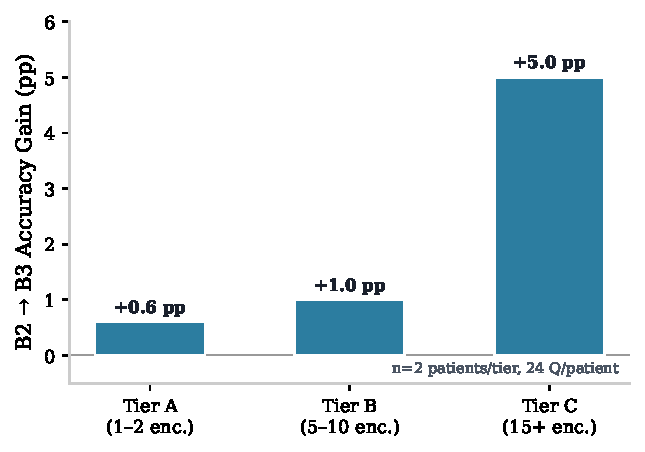
\includegraphics[width=0.75\textwidth]{figures/fig3_complexity_bars.pdf}
\vspace{4pt}
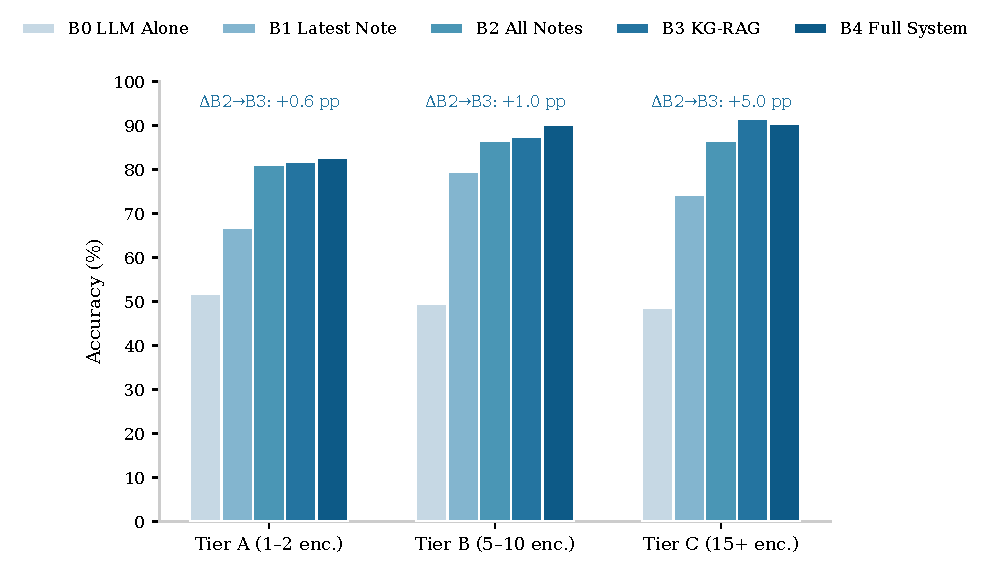
\includegraphics[width=\textwidth]{figures/fig4_waterfall.pdf}
\caption{SliceBench results ($n=2$ patients per tier, 24 questions each; point estimates without per-tier CIs). \textbf{Top:}~The KG layer's incremental benefit (B2$\rightarrow$B3) shows a directional, complexity-dependent trend: $+0.6\pp$ (Tier~A) to $+5.0\pp$ (Tier~C). \textbf{Bottom:}~Full condition progression by tier. The overall B2$\rightarrow$B3 delta is $+2.2\pp$ (CI: \ci{-1.5\pp}{+5.9\pp}).}
\label{fig:slicebench_figures}
\end{figure}


\section{Per-Category Delta Chart}
\label{app:deltas}

\begin{figure}[ht]
\centering
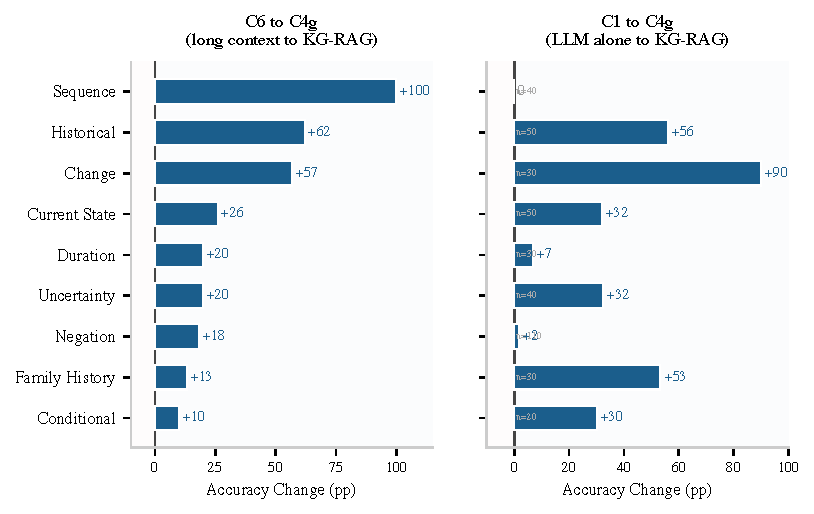
\includegraphics[width=\textwidth]{figures/fig5_category_deltas.pdf}
\caption{C1$\rightarrow$C4g per-category accuracy change. Intent-aware KG-RAG produces large gains on categories requiring cross-admission normalization (change, family history) and losses on categories where the LLM's parametric knowledge already suffices (historical, duration, conditional). Sample sizes per category shown.}
\label{fig:deltas}
\end{figure}


\section{SliceBench Conditions}
\label{app:slicebench_conditions}

\begin{table}[ht]
\centering
\small
\caption{SliceBench conditions. B0--B4 form a monotone context progression.}
\label{tab:slicebench_conditions}
\begin{tabular}{@{}clp{7.5cm}@{}}
\toprule
ID & Condition & Context Provided to LLM \\
\midrule
B0 & LLM Alone & Question only (parametric knowledge) \\
B1 & Latest Note & Most recent clinical note \\
B2 & All Notes RAG & All notes, retrieved by relevance \\
B3 & KG-RAG & Knowledge graph context + all notes \\
B4 & Full System & KG-RAG + guidelines + calculators \\
\bottomrule
\end{tabular}
\end{table}


\section{Supporting Results}
\label{app:supporting}

On MedQA-USMLE (965 questions), Claude Opus 4.5 achieves 81.6\% accuracy (5.1\,pp below GPT-4 at 86.7\% and Med-PaLM~2 at 86.5\%~\cite{medagentbench2025}), establishing that the Claude model family---Sonnet 4.5 (SliceBench answerer) and Opus 4.6 (ClinicalBench cross-model, SliceBench judge)---provides a reasonable LLM baseline.
Graph traversal latency is sub-millisecond at current scale (3,100 nodes, 8,803 edges): 0.57\,ms (1-hop), 0.75\,ms (2-hop).
The full system integrates 201 calculators, 1,202 guideline sections, 101 trigger patterns, and 24 edge types across 13 node types.


\section{DR.KNOWS Benchmark Results}
\label{app:drknows}

We evaluate \epikg on the DR.KNOWS diagnostic reasoning benchmark~\cite{drknows2025}, which measures knowledge graph traversal accuracy using real PostgreSQL-backed clinical data.

\begin{table}[ht]
\centering
\small
\begin{tabular}{lcc}
\toprule
\textbf{Metric} & \textbf{Score} & \textbf{\% of Baseline} \\
\midrule
Overall & 0.420 & 49.7\% \\
Path Discovery & 44.4\% & --- \\
Reasoning Accuracy & 22.2\% & --- \\
1-hop Traversal & 50.0\% & --- \\
2-hop Traversal & 25.0\% & --- \\
3-hop Traversal & 0.0\% & --- \\
\bottomrule
\end{tabular}
\caption{DR.KNOWS benchmark results. Multi-hop accuracy degrades due to PostgreSQL CTE limitations---an intentional tradeoff for ACID compliance.}
\label{tab:drknows}
\end{table}


\section{MedQA-USMLE Baseline}
\label{app:medqa}

\begin{table}[ht]
\centering
\small
\begin{tabular}{lccc}
\toprule
\textbf{Model} & \textbf{Accuracy} & \textbf{Step 1} & \textbf{N} \\
\midrule
EpiKG (LLM alone) & 81.6\% & 79.9\% & 965 \\
GPT-4 (2023) & 86.7\% & --- & 1{,}273 \\
Med-PaLM 2 (2023) & 86.5\% & --- & 1{,}273 \\
Claude 3 Opus (2024) & 78.0\% & --- & 1{,}273 \\
\bottomrule
\end{tabular}
\caption{MedQA-USMLE results. Our LLM-alone baseline is competitive.}
\label{tab:medqa}
\end{table}


\section{Scalability Metrics}
\label{app:scalability}

\begin{table}[ht]
\centering
\small
\begin{tabular}{lr}
\toprule
\textbf{Metric} & \textbf{Value} \\
\midrule
Documents processed & 145 \\
Patients & 85 \\
KG nodes & 3{,}100 \\
KG edges & 8{,}803 \\
1-hop traversal latency & 0.57\,ms \\
2-hop traversal latency & 0.75\,ms \\
\bottomrule
\end{tabular}
\caption{Scalability metrics at current deployment scale.}
\label{tab:scalability}
\end{table}


\section{System Component Scale}
\label{app:scale}

\begin{table}[ht]
\centering
\small
\begin{tabular}{lr}
\toprule
\textbf{Component} & \textbf{Scale} \\
\midrule
Clinical calculators & 201 \\
Guideline sections (RAG corpus) & 1{,}202 \\
OMOP vocabulary relationships & 20M+ \\
Assertion trigger patterns & 101 \\
KG edge types & 24 \\
KG node types & 13 \\
Assertion classes & 7 \\
\bottomrule
\end{tabular}
\caption{System component scale.}
\label{tab:system_scale}
\end{table}


\section{SliceBench Tier-Stratified Results}
\label{app:slicebench_tiers}

\begin{table}[ht]
\centering
\small
\caption{SliceBench results stratified by patient complexity tier. B2$\rightarrow$B3 $\Delta$ shows the incremental KG contribution.}
\label{tab:slicebench_tiers}
\begin{tabular}{@{}lccccccc@{}}
\toprule
& & \multicolumn{5}{c}{Score (\%)} & \\
\cmidrule(lr){3-7}
Tier & Encounters & B0 & B1 & B2 & B3 & B4 & B2$\rightarrow$B3 $\Delta$ \\
\midrule
A & 1--2 notes & 51.7 & 66.7 & 81.1 & 81.8 & 82.6 & $+0.6\pp$ \\
B & 5--10 notes & 49.5 & 79.4 & 86.4 & 87.4 & 90.1 & $+1.0\pp$ \\
C & 15+ notes & 48.4 & 74.2 & 86.5 & 91.5 & 90.3 & $+5.0\pp$ \\
\bottomrule
\end{tabular}
\end{table}


\section{ClinicalBench Full Per-Category Results}
\label{app:percategory}

\begin{table}[ht]
\centering
\small
\begin{tabular}{lcccccc}
\toprule
\textbf{Category} & \textbf{C1} & \textbf{C2} & \textbf{C3} & \textbf{C4} & \textbf{C4g} & \textbf{C5} \\
\midrule
Negation & 100.0 & 93.6 & 81.8 & 100.0 & 86.4 & 98.2 \\
Conditional & 100.0 & 90.0 & 55.0 & 70.0 & 65.0 & 75.0 \\
Uncertainty & 37.5 & 2.5 & 7.5 & 57.5 & 32.5 & 40.0 \\
Family History & 0.0 & 0.0 & 53.3 & 70.0 & 56.7 & 56.7 \\
Sequence & 80.0 & 80.0 & 80.0 & 87.5 & 90.0 & 77.5 \\
Current State & 64.0 & 54.0 & 50.0 & 54.0 & 76.0 & 58.0 \\
Duration & 100.0 & 100.0 & 83.3 & 83.3 & 46.7 & 73.3 \\
Historical & 94.0 & 78.0 & 68.0 & 60.0 & 40.0 & 68.0 \\
Change & 0.0 & 0.0 & 3.3 & 3.3 & 60.0 & 3.3 \\
\midrule
\textbf{Overall} & \textbf{71.5} & \textbf{62.5} & \textbf{59.2} & \textbf{71.5} & \textbf{66.0} & \textbf{68.2} \\
\bottomrule
\end{tabular}
\caption{Complete ClinicalBench per-category accuracy (\%, deterministic keyword evaluator) for all six conditions.}
\label{tab:full_percategory}
\end{table}


\section{Human Validation Pilot}
\label{app:human}

To assess LLM-as-judge reliability, we conducted a pilot validation study with a single board-certified physician who scored system outputs on a 4-point scale without knowledge of condition labels.
The pilot ($n=5$) revealed overly strict automated scoring on uncertainty and sequence questions. Gold standards were fully correct in 3/5 cases; model answers were partially correct or better in 3/5 cases where the auto-scorer marked them incorrect.
A full two-physician blinded adjudication ($n \geq 30$) is planned but not yet complete.


\section{Reproducibility Details}
\label{app:reproducibility}

\paragraph{Models.} ClinicalBench main ablation: MedGemma 27B via Ollama with deterministic keyword evaluator. Cross-model: MedGemma 27B and Claude Opus 4.6 (claude-opus-4-20250514) with the same evaluator. SliceBench: Claude Sonnet 4.5 (claude-sonnet-4-5-20250929, answering), Claude Opus 4.6 (judging). Temperature 0 throughout.

\paragraph{Evaluation.} The keyword evaluator matches temporal and assertion keywords against gold-standard categories, strips echoed evidence preambles, and includes expanded uncertainty keywords (medical hedging terms).

\paragraph{Bootstrap.} $n=2{,}000$ resamples, seed 42, BCa method~\cite{efron1993bootstrap}.

\paragraph{Data.} De-identified MIMIC-IV clinical notes under PhysioNet Credentialed Health Data Use Agreement~(v1.5.0).

\paragraph{Compute.} ClinicalBench: $\sim$3.6h (single GPU); Opus cross-model: $\sim$20min (API); SliceBench: $\sim$2h (API).

\paragraph{Evaluator evolution.} Key refinements: (i)~substring to word-boundary matching, (ii)~evidence preamble stripping. All main-text numbers use the final version.


\section{Assertion Category Definitions}
\label{app:assertions}

\begin{table}[ht]
\centering
\small
\begin{tabular}{lp{6.5cm}l}
\toprule
\textbf{Assertion} & \textbf{Definition} & \textbf{Example} \\
\midrule
\textsc{present} & Condition currently affirmed & ``has diabetes'' \\
\textsc{absent} & Condition explicitly negated & ``denies chest pain'' \\
\textsc{possible} & Condition suspected, not confirmed & ``possible pneumonia'' \\
\textsc{conditional} & Contingent on specific circumstances & ``if febrile, start antibiotics'' \\
\textsc{hypothetical} & Discussed as a scenario & ``would need dialysis if\ldots'' \\
\textsc{family\_history} & Attributed to a family member & ``mother had breast cancer'' \\
\textsc{historical} & Previously true, not necessarily current & ``former smoker'' \\
\bottomrule
\end{tabular}
\caption{The 7-value assertion taxonomy, extending i2b2 by separating \textsc{historical} from \textsc{family\_history}.}
\label{tab:assertion_defs}
\end{table}


\section{Intent-Aware Routing Algorithm}
\label{app:routing}

The C4g classifier is rule-based, mapping questions to \textsc{Change}, \textsc{Current\_State}, \textsc{Historical}, or \textsc{Default} using keyword patterns (e.g., ``changed'', ``new since'' trigger \textsc{Change}).
For \textsc{Change}, edges are partitioned by \texttt{hadm\_id} and set differences computed. For \textsc{Current\_State}, edges are filtered to current validity and deduplicated. For \textsc{Historical}, edges with past temporality are augmented with admission-based inference. Default questions use the C4 pipeline.


\section{C5 Full System Methodology}
\label{app:c5}

C5 extends C4 with guideline retrieval (1{,}202 sections) and clinical calculators (201, \eg CHA$_2$DS$_2$-VASc, MELD).
C5 achieves 68.2\% overall, below C1 and C4 (71.5\% each), likely because non-relevant components dilute the context window.


\section{Ethics Statement}
\label{app:ethics}

This work uses de-identified clinical data from MIMIC-IV~\cite{johnson2023mimiciv} under a PhysioNet Credentialed Health Data Use Agreement. No patient re-identification was attempted. The system is designed for clinical decision \emph{support}, not autonomous clinical decision-making.
